

\title[概率论]{第七讲: 全概率公式与贝叶斯公式}
%\author[张鑫 {\rm Email: xzhangseu@seu.edu.cn} ]{\large 张 鑫}
\institute[东南大学数学学院]{\large \textrm{Email: xzhangseu@seu.edu.cn} \\ \quad  \\
	\large 东南大学\quad 数学学院\\
	\vspace{0.3cm}
	%\trc{ 公共邮箱: \textrm{zy.prob@qq.com}\\
		% \hspace{-1.7cm}  密\qquad 码: \textrm{seu!prob}}
}
\date{}

{\setbeamertemplate{footline}{}
	\begin{frame}
		\titlepage
	\end{frame}
}
\subsection{全概率公式}

\begin{frame}{全概率公式的引入}
%	\begin{itemize}
%		\item 我们经常会碰到一些较为复杂的概率计算问题, 这时, 要对它们进行分解, 使之成为一些较为容易计算的情况, 以分别考虑, 全概率公式就是一个解决诸如此类复杂问题的有力武器.
%	\end{itemize}

	\begin{exam}
		有两个罐子
			\begin{itemize}[<+-|alert@+>]
			\item 在第一个罐中放有$7$个红球、$2$个白球和$3$个黑球
			\item 在第二个罐中放有$5$个红球、$4$个白球和$3$个黑球
			\item 从第一个罐中随机取出$1$个球放入第二个罐中
			\item 再从第二个罐中随机取出$1$个球来
			\item 试求$B$=\{从第二个罐中随机取出的球为红球\}的概率
		\end{itemize}
	\end{exam}
	\pause
	 \textcolor{cyan}{问题简要分析:}
	\begin{itemize}[<+-|alert@+>]
		\item 从第二个罐中随机取出的球这一随机试验结果依赖于第一次从第一个罐中所取球的结果;
		\item 因此,无论是计算$|B|$还是直接计算$P(B)$都不很容易
		\item 若已知第一次从第一个罐中所取球的结果后,则从第二个罐中随机取出的球为红球的概率很容易计算.
	\end{itemize}
\end{frame}

\begin{frame}{全概率公式的引入}
	\begin{jieda}
	\begin{itemize}[<+-|alert@+>]
		\item 以$A_1,A_2,A_3$分别表示由第一个罐子取出的是红球,白球和黑球;
		\item 显然$A_k, k=1,2,3$两两互不相容且$\bigcup_{k=1}^3A_k=\Omega$;
		\item $B=\bigcup_{k=1}^{3}A_kB\,$;
		\item $ P(B)=\sum_{k=1}^{3} P(A_kB)=\sum_{k=1}^{3} P(A_k) P(B|A_k)$;
		\begin{itemize}
			\item $ P(A_1)=\dfrac{7}{12},\, P(A_2)=\dfrac{1}{6},\, P(A_3)=\dfrac{1}{4}$;
			\item $ P(B|A_1)=\dfrac{6}{13},\, P(B|A_2)=\dfrac{5}{13},\, P(B|A_3)=\dfrac{5}{13}$;
		\end{itemize}
	\item 故$ P(B)=\dfrac{7}{12}·\dfrac{6}{13}+\dfrac{1}{6}·\dfrac{5}{13}+\dfrac{1}{4}·\dfrac{5}{13}=\dfrac{67}{156};$
	\end{itemize}
	\end{jieda}
\end{frame}

\begin{frame}
  \frametitle{全概率公式}
  \begin{thm}[\textcolor{red}{全概率公式}] 设$A_1,A_2,\cdots,A_n$为样本空间$\Omega$的一个分割, 即$A_1,\cdots,A_n$互不相容, 且$\cup_{k=1}^nA_k=\Omega$, 若$P(A_k)>0, k=1,2,\cdots,n$, 则对任一事件$B$有
    \begin{eqnarray*}
      P(B)=\sum_{k=1}^nP(A_k)P(B|A_k)
    \end{eqnarray*}
    \pause \zheng 因为
    \begin{eqnarray*}
      B=B\Omega=B(\cup_{k=1}^nA_k)=\cup_{k=1}^n(BA_k)
    \end{eqnarray*}
    \pause 且$BA_1,BA_2,\cdots,BA_n$互不相容, 所以由有限可加性得
    \pause
    \begin{eqnarray*}
      P(B)&=&P(\cup_{k=1}^n(BA_k))=\sum_{k=1}^nP(BA_k)\\ \pause
          &=&\sum_{k=1}^nP(A_k)P(B|A_k)\pause
    \end{eqnarray*}
  \end{thm}
\end{frame}



\begin{frame}{全概率公式图示}
    \begin{figure}[全概率公式.png]
      \centering
      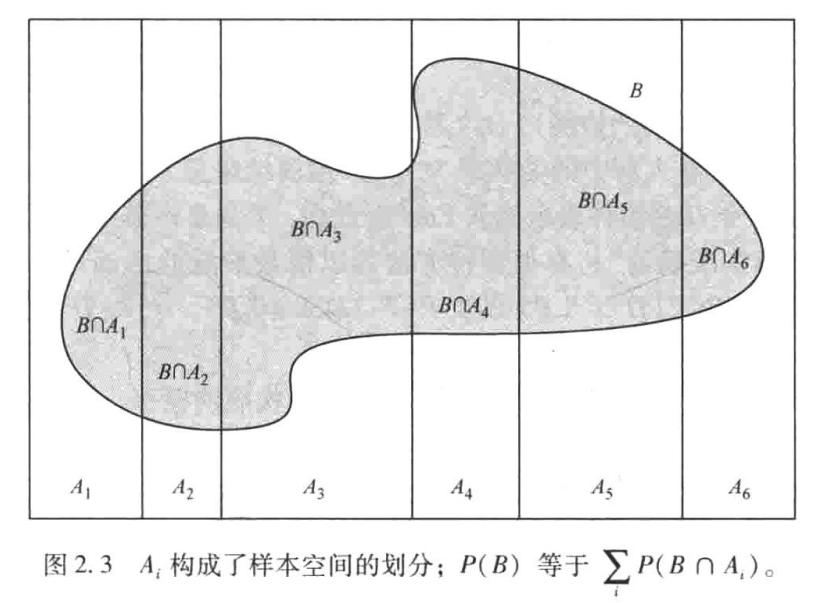
\includegraphics[width=7.5cm]{figures/全概率公式.png}
    \end{figure}

\end{frame}
\begin{frame}
  \frametitle{全概率公式( 续)}
  对于全概率公式, 我们要注意以下几点
  \begin{itemize}[<+-|alert@+>]
  \item 全概率公式的最简单形式: 如果$0<P(A)<1$, 则
    \begin{eqnarray*}
      P(B)=P(A)P(B|A)+P(\overline{A})P(B|\overline{A})
    \end{eqnarray*}
  \item 条件$A_1,A_2,\cdots,A_n$为样本空间$\Omega$的一个分割, 可改为$A_1,A_2,\cdots,A_n$互不相容, 且$B\subset \cup_{k=1}^nA_k$
  \item 在必要时,可把分割的概念推广到可列个事件($n=\infty$)的情形, 相应地有\pause
  $$ P(B)=\sum_{k=1}^{\infty} P(A_kB)=\sum_{k=1}^{\infty} P(A_k) P(B|A_k).$$
  \end{itemize}
\end{frame}



\subsection{贝叶斯公式}
\begin{frame}
	\frametitle{贝叶斯公式}
	\begin{thm}
		设$A_1,A_2,\cdots,A_n$为样本空间$\Omega$的一个分割, 即 $A_1,A_2,\cdots,A_n$互不相容, 且$\cup_{k=1}^nA_k=\Omega$, 若 $$P(B)>0, P(A_k)>0, k=1,2,\cdots,n$$ 则
		\begin{eqnarray*}
			P(A_k|B)=\dfrac{P(A_k)P(B|A_k)}{\sum_{j=1}^nP(A_j)P(B|A_j)}.
		\end{eqnarray*}
	特别的, 我们有
  \begin{eqnarray*}
    P(A|B)=\frac{P(B|A)P(A)}{P(B)}
    \end{eqnarray*}
	\end{thm}
\end{frame}


\begin{frame}{贝叶斯几率}
    \begin{defi}({\tc 几率}) 一个事件的几率(odds)为
    \begin{eqnarray*}
     ​\text{odds}(A)=P(A)/P(A^{\mathrm{c}})=\frac{P(A)}{1-P(A)}
     \end{eqnarray*}
    \end{defi}
  %\vspace{-0.5cm}
  \pause
  %\begin{itemize}[<+-|alert@+>]
  %\item
  \textcolor{cyan}{概率的几率表示:} $P(A)=\text{odds}(A)/(1+\text{odds(A)}) $
  %\end{itemize}
  \begin{thm} ({\tc 贝叶斯公式的几率形式})对于任意两个正概率事件$A$和$B$, 给定以$B$为条件的情况下, $A$的几率如下:
   \begin{eqnarray*}
    \frac{P(A|B)}{P(A^c| B)}=\frac{P(B| A)P(A)}{P(B| A^c)P(A^c)}
    \end{eqnarray*}
    \end{thm}
  \pause

  \begin{itemize}[<+-|alert@+>]
  \item 后验几率 $\dfrac{P(A|B)}{P(A^c|B)}$ 等于先验几率 $\dfrac{P(A)}{P(A^c)}$ 乘以似然比因子 $\dfrac{P(B|A)}{P(B|A^c)}$. % 这个因子就是统计学中很有名的似然比.
  \item 有时候用上述形式的贝叶斯准则可以更方便地求出后验几率, 如果需要的话还可以将几率形式转换成概率形式形式.
  \end{itemize}


\end{frame}




\begin{frame}{全概率与贝叶斯内涵:由因到果,由果推因}
	\begin{itemize}[<+-|alert@+>]
		\item 在现实中把事件$B$看作结果, 把事件$A_1,A_2,\cdots, A_n$看作导致结果$B$的各种原因
		\item 全概率公式是由各种原因推理出结果事件发生的概率,是由因到果
		\item 在日常生活中常常是观察到某种现象,反推造成这种现象的各种原因的概率,即由果推因
		\item 条件概率$P(A_k|B)$, 就是在观察到结果事件$B$已经发生的情况下,推断结果事件$B$是由原因$A_k$造成的概率的大小
		\item $P(A_k)$: 先验概率, 在没有别的前提信息情况下的概率值,一般借助经验来估计,或赋予所有原因以相同的先验概率
		\item $P(A_k|B)$:后验概率, 在获得“结果事件$B$发生”这个信息之后原因$A_k$出现的概率
		\item 后验概率可看作先验概率在获取了新信息之后的一种修正, 贝叶斯公式恰恰提供了一种计算后验概率的工具

%		\item 条件概率$P(A_k|B)$通常由贝叶斯公式来计算%Bayes 公式虽然很简单, 但是它却很有哲理意义
%	%	事件原因的事前可能性估计(先验概率$P(A_k)$)$\Rightarrow$得知结果后对可能性作出新的认识(后验概率$P(A_k|B)$)
%		\item Bayes
%		\item Bayes 学派: 对概率统计问题有自己的独特理解, 但他们主张按照同等无知原则, 赋予所有原因以相同的先验概率, 常受批评
%		\item 后来有人为了取其之长避其之短, 发展出所谓经验 Bayes 方法
%		\item 在计算机广为普及的今天, Bayes 方法和经验 Bayes 方法的实用价值也随之大大提高
		\item 贝叶斯理论对于人工智能、深度学习等理论具有重要的指导意义, 贝叶斯统计受到了从未有过的青睐, 迎来了前所未有的发展机遇
	\end{itemize}
\end{frame}

\begin{frame}
  \frametitle{条件全概率公式和条件贝叶斯公式}
  \vspace{0.2cm}
    \begin{thm} ({\tc 条件全概率公式}) 令$A_1,\cdots,A_n$为样本空间$\Omega$的一个划分. 设对于所有的$i$满足$P(A_iE)>0$, 则
   \begin{eqnarray*}
    P(B| E)=\sum_{i=1}^{n}P(B| A_{i},E)P(A_{i}| E)
    \end{eqnarray*}
    \end{thm}
    \pause
  \vspace{0.3cm}
  \begin{thm} ({\tc 条件贝叶斯公式}) 设$P(AE)>0$且$P(BE)>0$,则有
   \begin{eqnarray*}
    P(A| B,E)=\frac{P(B| A,E)P(A| E)}{P(B| E)}
    \end{eqnarray*}
    \end{thm}

\end{frame}
\subsection{全概率公式的应用}
\begin{frame}{全概率公式的应用}
	\begin{exam}
		有三个罐子, 各装有两个球, 分别为两个白球、一白一黑和两个黑球. 任意取出一个罐子, 摸出一球, 发现是白球. (1)求该罐中另一个球也是白球的概率; (2)把摸出的球放回罐中, 再从该罐中随机摸出一球, 求该球也是白球的概率.
	\end{exam}

	\begin{jieda}
		\begin{itemize}[<+-|alert@+>]
			\item $A_k, k=1,2$:表示第$k$次取球取出的是白球的事件;
			\item $B_k, k=1,2,3$:表示取出的是装有两白、一白一黑和两黑球的罐子;
			\item 问题(1)要求的是该白球取自两白的罐子的概率, 即$P(B_1|A_1)$;
			\item 由条件概率公式, 得$P(B_1|A_1)=\frac{P(A_1B_1)}{P(A_1)}=\frac{P(B_1)P(A_1|B_1)}{P(A_1)};$%=\frac{1/3}{1/2}=\frac{2}{3}.
			\begin{itemize}[<+-|alert@+>]
				\item $P(B_1)=1/3$, \pause $P(A_1|B_1)=1$;\pause
				\item $P(A_1)=\sum\limits_{k=1}^{3}P(B_k)P(A_1|B_k)=\dfrac{1}{3}\cdot 1+\dfrac{1}{3}\cdot\dfrac{1}{2}+\dfrac{1}{3}\cdot 0=\dfrac{1}{2}.$
			\end{itemize}
			\item $P(B_1|A_1)=\dfrac{1/3\cdot 1}{1/2}=2/3$.
		\end{itemize}

	\end{jieda}
\end{frame}

\begin{frame}{全概率公式的应用}
	\begin{itemize}[<+-|alert@+>]
	\item 问题(2)是在同一个罐子两次有放回的取球, 要求的是在第一次取出白球的条件下, 第二次取出的还是白球的条件概率, 即$P(A_2|A_1)$
	\item 由条件概率的定义, 知\pause $P(A_2|A_1)=\frac{P(A_1A_2)}{P(A_1)}$;\pause %$=\frac{5/12}{1/2}=\frac{5}{6}.$为此, 先要用全概率公式求出$P(A_1A_2)$:
	\begin{itemize}[<+-|alert@+>]
		\item $P(A_1)=\sum\limits_{k=1}^{3}P(B_k)P(A_1|B_k)=\dfrac{1}{3}·1+\dfrac{1}{3}·\dfrac{1}{2}+\dfrac{1}{3}·0=\dfrac{1}{2}.$
		\item $P(A_1A_2)=\sum\limits_{k=1}^{3}P(B_k)P(A_1A_2|B_k)=\dfrac{1}{3}·1+\dfrac{1}{3}·\dfrac{1}{4}+\dfrac{1}{3}·0=\dfrac{5}{12}.$
	\end{itemize}
	\item 	$P(A_2|A_1)=\frac{P(A_1A_2)}{P(A_1)}=\dfrac{5/12}{1/2}=\dfrac{5}{6}.$
\end{itemize}
\end{frame}
\begin{frame}{摸球问题}
	\begin{exam}
		甲盒中有球$5$红$1$黑, 乙盒中有球$5$红$3$黑. 随机取出一个盒子, 从中无放回地相继取出两个球, 试求在第一个球是红球的条件下, 第二个球也是红球的概率.
	\end{exam}
	\pause

	\begin{jieda}
		\begin{itemize}[<+-|alert@+>]
			\item $B:=$\{第一个球是红球\}, $C:=$\{第二个球是红球\}
			\item $P(C|B)=\pause \dfrac{P(BC)}{P(B)}$ \pause
			\begin{itemize}[<+-|alert@+>]
				\item $A:=$\{取出的是甲盒\}
				\item $P(BC)=\pause P(A)P(BC|A)+P(\overline{A})P(BC|\overline{A})=\pause \dfrac{1}{2}·\dfrac{5}{6}·\dfrac{4}{5}+\dfrac{1}{2}·\dfrac{5}{8}·\dfrac{4}{7}=\dfrac{43}{84}$


				\item $P(B)=\pause P(A)P(B|A)+P(\overline{A})P(B|\overline{A})=\pause \dfrac{1}{2}·\dfrac{5}{6}+\dfrac{1}{2}·\dfrac{5}{8}=\dfrac{35}{48}$%于是$\overline{A}$即为取出的是乙盒的事件. 由条件概率公式和全概率公式知
				%			\begin{align*}
					%				P(C|B)&=\frac{P(BC)}{P(B)}=\frac{P(A)P(BC|A)+P(\overline{A})P(BC|\overline{A})}{P(A)P(B|A)+P(\overline{A})P(B|\overline{A})}\\
					%				&=\frac{\dfrac{1}{2}·\dfrac{5}{6}·\dfrac{4}{5}+\dfrac{1}{2}·\dfrac{5}{8}·\dfrac{4}{7}}{\dfrac{1}{2}·\dfrac{5}{6}+\dfrac{1}{2}·\dfrac{5}{8}}=\frac{172}{245}.
					%			\end{align*}
			\end{itemize}
			\item $P(C|B)=\dfrac{43}{84}/\dfrac{35}{48}=\dfrac{172}{245}$
		\end{itemize}

	\end{jieda}
	%	\begin{itemize}
		%		\item 在该例的计算中, 分子与分母都用到了全概率公式
		%	\end{itemize}
\end{frame}


%\begin{frame}{全概率公式的应用}
%	\begin{jieda}
%		于是由全概率公式知
%		$$P(E)=P(B)P(E|B)+P(B^c)P(E|B^c)=\frac{1}{2}\left(P(A_0)+P(A_1)+P(A_2)\right)=\frac{1}{2}.$$
%	\end{jieda}
%	\begin{itemize}
%		\item 应当注意, 根据对称性, 我们可以得出: 乙抛出的反面比甲多的概率也是$\dfrac{1}{2}$; 而不是: 乙抛出的正面比甲少的概率等于$\dfrac{1}{2}$.
%	\end{itemize}
%\end{frame}
\begin{frame}
	\frametitle{一般摸球模型}
	\begin{exam}
		袋中有$r$个红球与$b$个黑球. 每次从袋中任摸出 1 球并连同$s$个同色球一起放回. 以$R_n$表示第$n$次摸出红球, 试证$P(R_n)=\dfrac{r}{r+b}$.
	\end{exam}

	\pause
	\zheng 利用归纳法来证明:$n=1$时, $P(R_1)=\dfrac{r}{r+b}$显然成立.

	\pause 假设$n-1$时命题成立. 为求$P(R_n)$, 我们以第 1 次取球的可能结果$R_1$与$\bar{R}_1$作为$\Omega$的分割, 用全概率公式可得:
	\pause
	\begin{align*}
		P(R_n)&=\pause P(R_1)P(R_n|R_1)+P(\bar{R}_1)P(R_n|\bar{R}_1)\\
		&= \pause\dfrac{r}{r+b}\cdot \dfrac{r+s}{r+s+b}+\dfrac{b}{r+b}\cdot \dfrac{r}{r+b+s}\\
		&=\pause\dfrac{r}{r+b}
	\end{align*}
	\pause
	\begin{rmk}
		当$s=0$时相当于放回摸球, 而$s=-1$相当于不放回摸球.
	\end{rmk}

\end{frame}




\begin{frame}{Simpson 悖论}
	\begin{exam}
		有两种治疗肾结石的方案,其治疗效果如下:
		\begin{itemize}[<+-|alert@+>]
			\item \textcolor{cyan}{方案$1$:} 小结石患者占$25\%$, 大结石患者占$75\%$, 小结石患者的治愈率是$93\%$, 大结石患者的治愈率是$73\%$
			\item \textcolor{cyan}{方案$2$:} 小结石患者占$77\%$, 大结石患者占$23\%$, 小结石患者的治愈率是$87\%$, 大结石患者的治愈率是$69\%$
			\item 不管是对小结石患者, 还是大结石患者, 方案$1$的治愈率都要高于方案$2$
			\item \textcolor{red}{方案$1$优于方案$2$吗?}
		\end{itemize}
	\end{exam}
	\pause
	\begin{jieda}
		计算两种方案的治愈率
		\begin{itemize}[<+-|alert@+>]
			\item 记$A$=\{患者是小结石患者\}, $B$=\{患者被治愈\}
			\item 根据全概率公式\pause
			\begin{align*}
				&\hspace{-0.5cm}P_1(B)=\pause P_1(A)P_1(B|A)+P_1(\overline{A})P_1(B|\overline{A})=\pause 0.25·0.93+0.75·0.73=0.78\pause \\
				&\hspace{-0.5cm} P_2(B)=\pause P_2(A)P_2(B|A)+P_2(\overline{A})P_2(B|\overline{A})=\pause 0.77·0.87+0.23·0.69=0.8286
			\end{align*}
			\item 方案$2$的治愈率高于方案$1$, 可见方案$1$并不优于方案$2$
		\end{itemize}
	\end{jieda}
\end{frame}

\begin{frame}
	\frametitle{敏感性问题调查}
	敏感性问题调查方案的关键在于要使被调查者愿意作出真实的回答又能保守个人秘密, 如果调查方案有误, 被调查者就会拒绝配合, 所得调查数据将失去真实性.
	\pause
	\vspace{0.5cm}

	{\bf 调查方案: } 被调查者只需要加答以下两个问题中的一个问题,且只需要回答“是”或“否”.

	\pause
	问题 A: 你的生日是否在 7 月 1 日之前?

	问题 B: 所调查的敏感性问题.

	\pause
	\vspace{0.5cm}
	{\bf 调查方案的操作: }

	( 1)被调查者在没有旁人的情况下独自一人在房间内操作回答问题

	\pause
	( 2)被调查者从一个罐子中随机抽一球, 看过颜色后放回, 若抽到白球, 回答问题 A, 抽到红球, 回答问题 B.

	( 3)被调查者无论回答问题 A 还是问题 B, 只需在仅有“是”与“否”选项的答卷上作答然后将答卷放入密封的投票箱内.

\end{frame}

\begin{frame}
	\frametitle{敏感性问题调查}
	{\bf \textcolor{red}{问题:}} 假若我们有$n$张问卷, 其中$k$张回答“是”, 我们如何确定选定红球回答问题 B 为“是”的概率?


	\pause
	{\bf \textcolor{red}{已知:}}
	\begin{itemize}[<+-|alert@+>]
		\item 红白球的比例, 即$P(\mbox{红球}):=\pi, P(\mbox{白球})=1-\pi$;
		\item $P(\mbox{是}|\mbox{白球})=0.5$;
		\item $P(\mbox{是})\approx \dfrac{k}{n}$.
	\end{itemize}
	\pause
	{\bf \textcolor{red}{待求:}} $p:=P(\mbox{是}|\mbox{红球})$.

	\pause
	{\bf\jieda} 由全概率公式可得
	\begin{eqnarray*}
		P(\mbox{是})=P(\mbox{白球})P(\mbox{是}|\mbox{白球})+P(\mbox{红球})P(\mbox{是}|\mbox{红球})
	\end{eqnarray*}
	即\pause
	\begin{eqnarray*}
		\dfrac{k}{n}\approx (1-\pi)\cdot 0.5+\pi\cdot p \Rightarrow p=\dfrac{k/n-0.5(1-\pi)}{\pi}
	\end{eqnarray*}


\end{frame}



\begin{frame}{掷硬币问题}
	\begin{exam}
		甲、乙二人抛掷一枚均匀的硬币, 甲抛了$100$次, 乙抛了$101$次. 求事件$E:=$\{乙抛出的正面次数比甲多\}的概率.
	\end{exam}

	\begin{jieda}
		\begin{itemize}[<+-|alert@+>]
			\item 如果甲和乙都抛掷这枚均匀的硬币$100$次, 那么当然会有三种不同的可能结果
			\begin{itemize}[<+-|alert@+>]
				\item $A_0$:\pause 甲乙抛出的正面次数一样多\pause
				\item $A_1$:\pause 甲抛出的正面次数比乙多\pause
				\item $A_2$:\pause 乙抛出的正面次数比甲多\pause
				\item $P(A_0)+P(A_1)+P(A_2)=1$\pause 且 $P(A_1)=P(A_2)$\pause
			\end{itemize}
			\item 以乙第一次抛出的硬币结果对样本空间进行分割:
			\begin{itemize}[<+-|alert@+>]
				\item 若$B=$\{乙第一次时抛出的是正面\}发生, 则\pause 乙只要在接下来的$100$次抛掷中, 抛出的正面次数不比甲少即可, 即
				\[P(E|B)=P(A_0)+P(A_1)\]
				\item 若$\overline{B}:=$\{乙第一次时抛出的是反面\}发生, 则\pause 乙只要在接下来的$100$次抛掷中, 抛出的正面次数比甲多即可, 即$P(E|\overline{B})=P(A_1)=P(A_2)$
			\end{itemize}
			\item $P(E)=P(B)P(E|B)+P(\overline{B})P(E|\overline{B})=\frac{1}{2}\left(P(A_0)+P(A_1)+P(A_2)\right)=\frac{1}{2}.$
		\end{itemize}
	\end{jieda}
\end{frame}




\begin{frame}{对战获胜概率问题}
	%	\begin{itemize}
		%		\item 全概率公式是一件有力的工具, 灵活地运用它往往会带来简洁有效的解法
		%	\end{itemize}
	\begin{exam}
		甲、乙进行某项对战比赛, 每回合胜者得$1$分, 败者不得分. 比赛进行到有 1 人比另外 1 人多$2$分终止, 多$2$分者获胜. 现知每回合甲胜的概率为$p\in (0,1)$. 试求$A:=$\{甲最终获胜\}的概率.
	\end{exam}

	\begin{jieda}
		\textcolor{red}{法一(经典解法)}
		\begin{itemize}[<+-|alert@+>]
			\item 显然甲只能在偶数个回合后获胜
			\item 记$A_{2n}$=\{甲在$2n$个回合后获胜\}, \pause 则$A=\cup_{n=1}^\infty A_{2n}$\pause
			\item $A_{2n}, n\geq 1$两两互不相容且\pause $P(A_{2n})=(2p(1-p))^{n-1}p^2$
			\item 甲最终获胜的概率
			\begin{align*}
				P(A)&=\sum_{n=1}^{\infty}P(A_{2n})=p^2\sum_{n=1}^{\infty}(2p(1-p))^{n-1}\\
				&=p^2\sum_{n=0}^{\infty}(2p(1-p))^{n}=\dfrac{p^2}{1-2p(1-p)}.
			\end{align*}
		\end{itemize}
	\end{jieda}
\end{frame}

\begin{frame}{对战获胜概率问题}
	\begin{jieda}
		\textcolor{red}{法二(全概率公式)}
		\begin{itemize}[<+-|alert@+>]
			\item 以前两个回合的战绩对样本空间进行分割
			\item 分别以$B_1,B_2,B_3$表示甲二胜、一胜一败、二败事件
			\item $P(B_1)=p^2,\,P(B_2)=2p(1-p),\,P(B_3)=(1-p)^2$
			\item $P(A|B_1)=1,\,P(A|B_2)=P(A),\,P(A|B_3)=0$
			\item 由全概率公式得$P(A)=\sum\limits_{i=1}^{3}P(B_i)P(A|B_i)=p^2+2p(1-p)P(A)$
			\item $P(A)=\dfrac{p^2}{1-2p(1-p)}$
		\end{itemize}
	\end{jieda}
\end{frame}

\begin{frame}{对战获胜概率问题}
	\begin{jieda}
		\textcolor{red}{法三(随机游动)}
		\begin{itemize}[<+-|alert@+>]
			\item 考察质点在数轴整数点上的随机游动:在整数点$x=n$
			\begin{itemize}[<+-|alert@+>]
				\item 以概率$p$向右移动到整数点$x=n+1$,
				\item 以概率$1-p$向左移动到整数点$x=n-1$
			\end{itemize}
			\item 以$p_n$表示“质点由$x=n$出发, 未达$-2$前先到达$2$的概率”
			\item 显然, $p_{-2}=0,p_2=1$
			\item 甲获胜的概率即为: $p_0$
			\item 由全概率公式易得
			\begin{equation}
				\left\{
				\begin{aligned}
					&p_0=pp_1+(1-p)p_{-1}, \pause \\ \notag
					&p_1=pp_2+(1-p)p_0=p+(1-p)p_0, \pause \\
					&p_{-1}=pp_0+(1-p)p_{-2}=pp_0.\pause
				\end{aligned}
				\right.
			\end{equation}\pause
			\item $p_0=p(p+(1-p)p_0)+(1-p)(pp_0)\pause =p^2+2p(1-p)p_0$\pause
			\item 故 $$p_0=\dfrac{p^2}{1-2p(1-p)}.$$
		\end{itemize}
	\end{jieda}
\end{frame}





\subsection{Bayes 公式的应用}
\begin{frame}{随机抛硬币问题}
	\begin{exam}({\tc 随机抛硬币}) 假设有一枚均匀的硬币和一枚以概率$3/4$正面朝上的不均匀硬币. 随机选取一枚硬币掷$3$次, $3$次都是正面朝上. 试问: %
		\vspace{-0.4cm}
	\begin{enumerate}[<+-|alert@+>]
		\item 给定上述信息后, 选取的硬币是均匀硬币的概率有多大?
		\item 接下去掷第四次时, 仍是正面朝上的概率是多少?
		\end{enumerate}
	\end{exam}
	\pause
%\vspace{-0.2cm}
\begin{jieda}
  令 \begin{align*}
	A &:=\{\mbox{选取的硬币掷 3 次均正面朝上}\}\\
	F & :=\{\mbox{选取的硬币是均匀的}\},\quad
	H :=\{\mbox{第 4 次正面朝上} \}
  \end{align*}
  则\pause
  {\small \begin{align*}
	P(F|A) \pause &=\frac{P(A|F)P(F)}{P(A)}\pause =\frac{P(A|F)P(F)}{P(A|F)P(F)+P(A|F^c)P(F^c)} \\
	\pause &=\frac{(1/2)^3 \cdot 1/2}{(1/2)^3 \cdot 1/2 +(3/4)^3 \cdot  1/2}\pause \approx 0.23\\
    P(H\mid A)\pause & =P(\left.H\mid F,A\right)P(\left.F\mid A\right)+P(\left.H\mid F^{\mathrm{c}},A\right)P(\left.F^{\mathrm{c}}\mid A\right)  \\
	\pause &=\frac{1}{2}\cdot0.23+\frac{3}{4}\cdot(1-0.23) \pause \approx 0.69.
  \end{align*}}
\end{jieda}



\end{frame}







\begin{frame}{罕见病检测诊断问题}
	\begin{exam}考虑以验血结果诊断某种罕见病的患病概率:
		\begin{itemize}[<+-|alert@+>]
			\item 	某罕见病的发病率为$1\%$
			\item 通过验血诊断该病的误诊率为$5\%$, 即非患者中有$5\%$的人验血结果为阳性, 患者中有$5\%$的人验血结果为阴性
			\item 现已知某人验血结果为阳性, 试求他患有此病的概率
		\end{itemize}
	\end{exam}
	\pause

	\begin{jieda}
		\begin{itemize}[<+-|alert@+>]
			\item 记$D:=$\{患有此病\}, $T_{1}:=$\{第一次验血结果为阳性\}.
			\item 要求的概率是: $P(D|T_{1})=\dfrac{P(DT_{1})}{P(T_{1})}=\dfrac{P(D)P(T_{1}|D)}{P(T_{1})}$
			\item 由题意可知%知条件知
			\begin{align*}
				P(D)&=1\%,\,P(\overline{D})=99\%, \, P(T_{1}|D)=95\%,\,P(T_{1}|\overline{D})=5\%\pause \\
				P(T_{1})&=P(D)P(T_{1}|D)+P(\overline{D})P(T_{1}|\overline{D})=1\%\cdot 95\%+99\%\cdot 5\% \pause \\
        &=0.0685\pause
			\end{align*}
		\end{itemize}
	\end{jieda}
\end{frame}

			\begin{frame}{罕见病检测诊断问题}
				\begin{itemize}[<+-|alert@+>]

			\item
			%		$D$和$\overline{D}$构成了对$\Omega$的分划, 故由 T_{1}ayes 公式得
			$P(D|T_{1})=\dfrac{P(D)P(T_{1}|D)}{P(T_{1})}=\dfrac{1\%\cdot 95\%}{0.0685}\approx 0.16.$
		    \item 几率方法:
			$$\frac{P(D|T_1)}{P(D^c|T_1)}=\frac{P(D)}{P(D^c)}\frac{P(T_1|D)}{P(T_1|D^c)}=\frac{1}{99}\cdot\frac{0.95}{0.05}\approx 0.19$$
			\pause
			由几率与概率之间的关系可知
			$$P(D|T_1)=0.19/(1+0.19)\approx 0.16, $$ 与上述结果一致.
			\item 用几率形式的贝叶斯准则计算更迅速的原因是此时不需要计算普通贝叶斯准则的分母.
		\end{itemize}
\end{frame}


\begin{frame}{罕见病检测诊断问题图示}
	\begin{figure}%[ch1-bayes-disease.png]
		\centering
		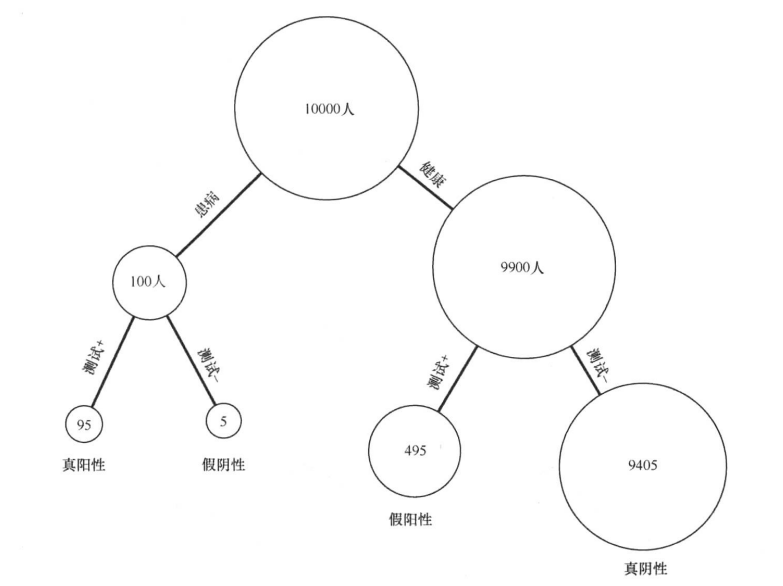
\includegraphics[width=10.5cm]{figures/ch1-bayes-disease.png}
	  \end{figure}

\end{frame}

\begin{frame}{罕见病检测诊断问题}
	\begin{exam} 接上例, 检测结果为阳性的某人, 决定进行第二次检测. 假设新的检测结果与之前的结果相互独立, 且有相同的敏感性和特异性. 若第二次检测结果也为阳性, 试求此人患有此病的概率.
	\end{exam}
	\pause

	\begin{jieda}
		\begin{itemize}[<+-|alert@+>]
			\item 记 %$D:=$\{患有此病\}, $T_{1}:=$\{第一次验血结果为阳性\}, \\ \quad
			$T_{2}:=$\{第二次验血结果为阳性\}
			\item 要求的概率是: $P(D|T_{1}T_{2})$%$=\dfrac{P(DT_{1})}{P(T_{1})}=\dfrac{P(D)P(T_{1}|D)}{P(T_{1})}$
			\item 一步法: 将两个检测结果一次性都考虑在内以进行概率更新,
			\begin{itemize}[<+-|alert@+>]
			\item 计算几率
            $$\frac{P(D|T_1\cap T_2)}{P(D^c|T_1\cap T_2)}=\frac{P(D)}{P(D^c)}\frac{P(T_1\cap T_2|D)}{P(T_1\cap T_2|D^c)}=\frac{1}{99}\cdot \frac{0.95^2}{0.05^2}=\frac{361}{99}\approx 3.646$$
			\item $P(D|T_{1}T_{2})=\frac{3.646}{1+3.646}\approx 0.78$.
			\end{itemize}
		\end{itemize}
	\end{jieda}
\end{frame}

\begin{frame}{罕见病检测诊断问题}
			\begin{itemize}[<+-|alert@+>]
			\item 两步法:
			\begin{itemize}[<+-|alert@+>]
			\item 在完成第一次检测后, 某人患有此病的后验几率为
             $$\frac{P(D|T_1)}{P(D^c|T_1)}=\frac{1}{99}\cdot\frac{0.95}{0.05}\approx 0.19$$
			 \item 将后验几率作为新的先验几率, 然后基于第二次检测结果更新后验几率%更新为
			 \begin{align*}
				\frac{P(D|T_1\cap T_2)}{P(D^c|T_1\cap T_2)}
				&=\frac{P(D|T_1)}{P(D^c|T_1)}\frac{P(T_2|D,T_1)}{P(T_2|D^c,T_1)}\\
				&=(\frac{1}{99}\cdot\frac{0.95}{0.05})\frac{0.95}{0.05}\\
				&=\frac{361}{99}\approx 3.646
			 \end{align*}

			\item $P(D|T_{1}T_{2})=\dfrac{3.646}{1+3.646}\approx 0.78$
			\end{itemize}

		\end{itemize}
\end{frame}


\begin{frame}{{\rm Monty Hall}三门问题}
  \begin{exam}在 Monty Hall 主持的“Let's Make a Deal”节目中, 有三扇门, 其中有两扇门后面是一只山羊, 一扇门后面是一辆车.  选手将获得其所选中的那扇门后面的物品.
	\begin{itemize}[<+-|alert@+>]
	\item 一位选手从三扇最近的门中选一扇
	\item Monty 知道车在哪扇门后面, 并以不暴露车的位置打开剩下两扇门中的一扇, 即他打开的门后面永远是山羊.
	\item 若剩下的两扇门后都是山羊的话, Monty 会等可能地随机选一扇门.
	\item 然后 Monty 会让对手选择, 是换另一扇没打开的门还是不换.
	\item 如果对手的目标是得到车, 她应该换吗?
	\end{itemize}

    \end{exam}
    \vspace{-0.2cm}
     \begin{figure}[Monty Hall 问题.png]
      \centering
      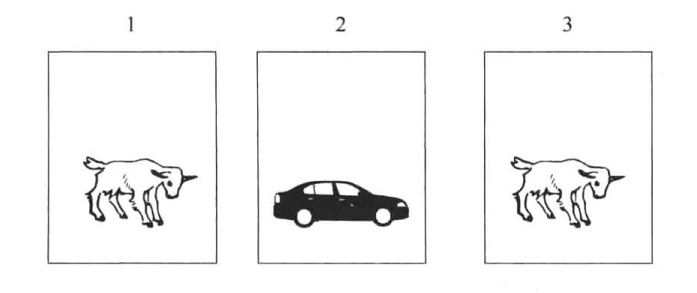
\includegraphics[width=8.5cm]{figures/Monty Hall 问题.png}
    \end{figure}
\end{frame}

\begin{frame}{Monty Hall 问题(续)}
\begin{jieda}
\begin{itemize}
\item 先将三扇门从$1$到$3$编号. \\
\item 不失一般性, 可以假设选手选择的是$1$号门
\item 令
\begin{align*}
	A&=\{\mbox{换门得到车} \} \\
	B&=\{\mbox{不换门得到车} \}\\
   C_i&:=\{\mbox{车在第}i \mbox{扇门后面} \}, i=1,2,3.
\end{align*}
\item 显然, $P(B)=P( \mbox{不换门得到车} )=1/3$

\item 则由全概率公式
\begin{align*}
	P(A)&=P(A|C_1)\cdot\frac{1}{3}+P(A|C_2)\cdot\frac{1}{3}+P(A|C_3)\cdot\frac{1}{3}\\
   & =0\cdot\frac{1}{3}+1\cdot\frac{1}{3}+1\cdot\frac{1}{3}=\frac{2}{3}
\end{align*}

\end{itemize}
\end{jieda}
\end{frame}

\begin{frame}{Monty Hall 三门问题图示}
	\begin{figure}[ch1-montyhall-visual-prob.png]
		\centering
		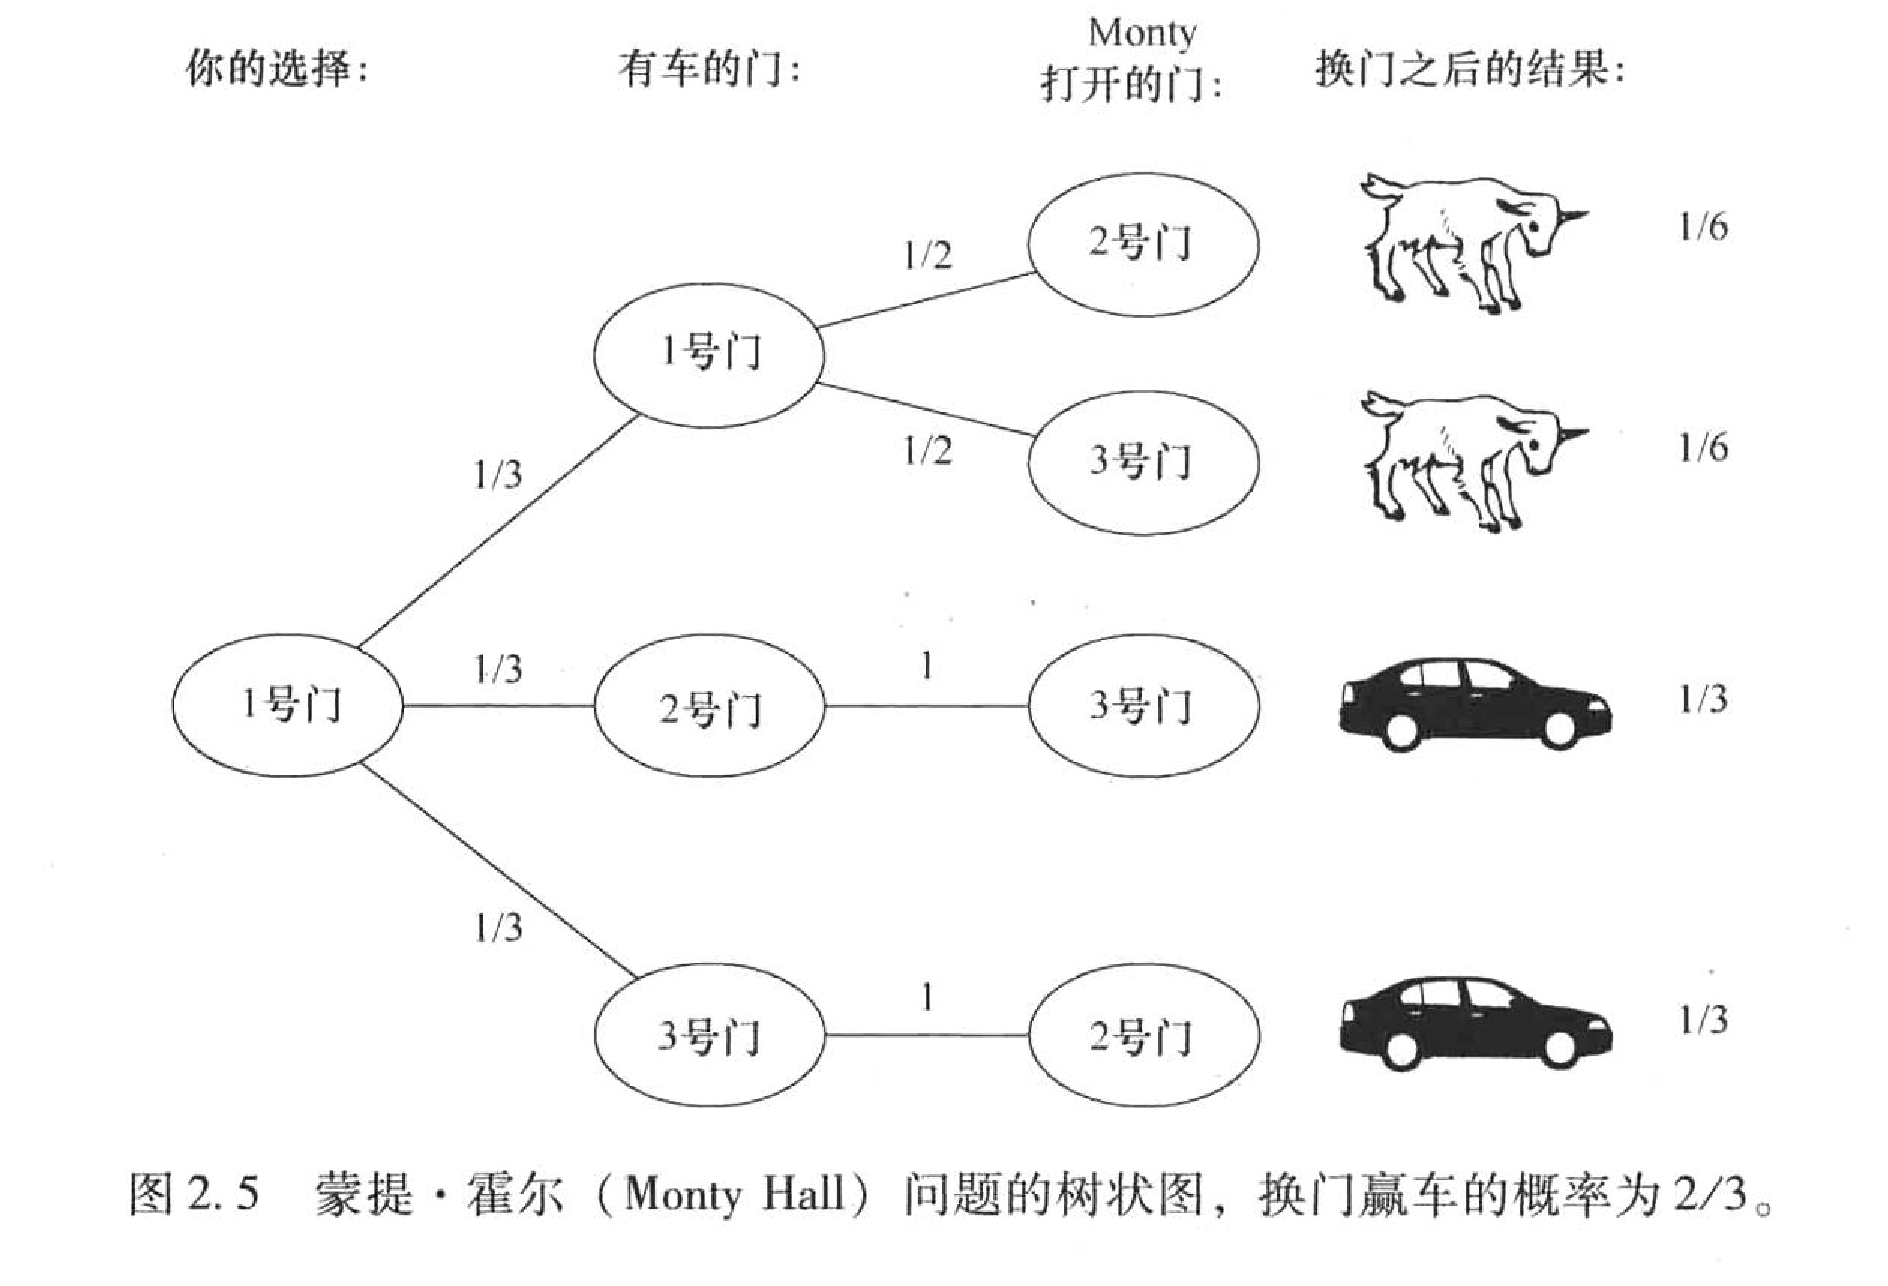
\includegraphics[width=11cm]{figures/ch1-montyhall-visual-prob.png}
	  \end{figure}

\end{frame}





%\begin{frame}{Bayes 公式的应用}
%	\begin{itemize}
	%		\item 这个结果出人意料的小, 其原因在于人群中该病的患病率很低, 仅为$0.5\%$, 所以尽管通过验血诊断该病的误诊率不算高, 为$5\%$ , 但与患病率相比己是$10$倍之多
	%		\item 当验血结果为阳性时, 确患有此病的概率并不一定就很大
	%		\item 患病的概率除了依赖于验血时的准确率之外, 还与人群中该病的患病率有关, 这一点对于罕见病的诊断尤为重要
	%	\end{itemize}
%\end{frame}
\begin{frame}{电邮问题}
	\vspace{-0.2cm}
	\begin{exam}
		甲、乙二人之间经常用 E-mail 相互联系, 他们约定在收到对方信件的当天即给 E-mail 回复. 由于线路问题, 每$n$份 E-mail 中会有$1$份不能在当天送达收件人. 甲在某日发了$1$份 E-mail 给乙, 但未在当天收到乙的回音. 试求乙在当天收到了甲发给他的 E-mail 的概率.
	\end{exam}
	\pause

	\begin{jieda}
		\begin{itemize}[<+-|alert@+>]
			\item 在这个问题中, 包含了两个不确定的环节:
			\begin{itemize}[<+-|alert@+>]
				\item 甲发给乙的 E-mail 不一定在当天到达乙处
				\item 乙回给甲的 E-mail 不一定在当天到达甲处
			\end{itemize}
			\item $A$=\{乙在当天收到甲的 E-mail\}, $B$=\{甲在当天收到乙回的 E-mail\}
			\item $P(A|\overline{B})=\dfrac{P(A)P(\overline{B}|A)}{P(A)P(\overline{B}|A)+P(\overline{A})P(\overline{B}|\overline{A})}$
			\item %$A$和$\overline{A}$构成了对$\Omega$的分划.
			由题中条件知
			$$P(A)=\frac{n-1}{n},\, P(\overline{A})=\frac{1}{n}, \,P(\overline{B}|A)=\frac{1}{n},\,P(\overline{B}|\overline{A})=1.$$
			\item $P(A|\overline{B})=\dfrac{\frac{n-1}{n}·\frac{1}{n}}{\frac{n-1}{n}·\frac{1}{n}+\frac{1}{n}·1}=\dfrac{n-1}{2n-1}<1/2$
		\end{itemize}
	\end{jieda}
\end{frame}
%\begin{frame}{Poly\'{a}罐子模型续}
%	\begin{exam}
%		罐中放有$a$个白球和$b$个黑球, 每次从罐中随机抽取一个球, 并连同$c$个同色球一起放回罐中, 如此反复进行. 试证明: 在第$n$次取球时取出白球的概率为$\dfrac{a}{a+b}$.
%	\end{exam}
%
%	\begin{jieda}
%		记$A_k$=\{在第$k$次取球时取出白球\}, 于是$A_k^c$=\{在第$k$次取球时取出黑球\}. 以下利用数学归纳法:
%
%		显然有$P(A_1)=\dfrac{a}{a+b}$成立. 假设$n=k-1,\,k\geq 2$时结论成立, 要证$n=k$时结论也成立.
%
%		以$A_1$和$A_1^c$作为对$\Omega$的一个分划, 此时可将$P(A_k|A_1)$看成从原来放有$a+c$个白球和$b$个黑球的罐中按规则取球, 并且在第$k-1$次取球时取出白球的概率, 因此由归纳假设知$P(A_k|A_1)=\dfrac{a+c}{a+b+c}$, 同理亦有$P(A_k|A_1^c)=\dfrac{a}{a+b+c}$.
%	\end{jieda}
%\end{frame}
%
%\begin{frame}{Poly\'{a}罐子模型续}
%	\begin{jieda}
%		于是由全概率公式得
%		\begin{align*}
%			P(A_k)&=P(A_1)P(A_k|A_1)+P(A_1^c)P(A_k|A_1^c)\\
%			&=\frac{a}{a+b}·\frac{a+c}{a+b+c}+\frac{b}{a+b}·\frac{a}{a+b+c}=\frac{a}{a+b}.
%		\end{align*}
%		因此, 结论对一切$n$成立.
%	\end{jieda}
%
%	\begin{itemize}
%		\item 本题解答中对$\Omega$的分划的选取方式值得注意
%		\item 易走的一条歧路是把$A_{k-1}$和$A_{k-1}^c$作为对$\Omega$的分划
%		\begin{itemize}
%			\item 在这种选取之下, 难以利用归纳假设算出条件概率$P(A_k|A_{k-1})$和$P(A_k|A_{k-1}^c)$, 因为此时只知道罐中有$a+b+(k-1)c$个球, 而难以知道白球和黑球的数目
%			\item 相反地, 在$A_1$和$A_1^c$发生的情况下, 罐中白球和黑球的数目十分清楚
%		\end{itemize}
%		\item 这个事实再次表明正确选取分划方式的重要性
%		\item 当然也要正确理解归纳假设
%	\end{itemize}
%\end{frame}

\subsection{条件化及计算概率的递推方法}

\begin{frame}{计算概率的递推方法: 一步分析}

 \begin{exam}{\tc (分支过程)}
池塘里只有一只变形虫叫作 Bobo.
\begin{itemize}[<+-|alert@+>]
\item  每过$1$分钟, Bobo 有三种结果: 死去、分裂成两个或保持原状
\item 三种结果出现的概率相同
\item  此后所有活着的 Bobo 都将继续以这种方式相互独立地进行下去
\item  那么这个变形虫种族最终灭亡的概率是多少?
\end{itemize}
\end{exam}
\vspace{-0.2cm}
     \begin{figure}[分支过程.png]
      \centering
      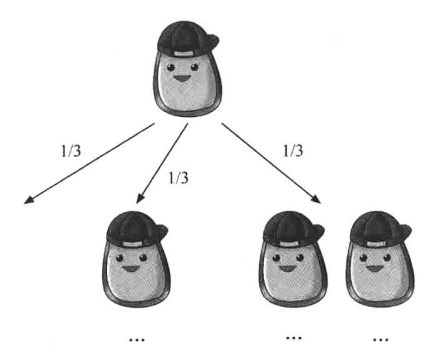
\includegraphics[width=6cm]{figures/分支过程.png}
    \end{figure}
\end{frame}

\begin{frame}{分支过程(续)}
\begin{jieda}
\begin{itemize}[<+-|alert@+>]
\item 令$D:=\{\mbox{最终种族灭绝}\}$, 本题希望求出$P(D)$.
\item 我们在第一步结果的基础上即以$1$分钟后的结果进行分析:
\begin{itemize}[<+-|alert@+>]
\item 令$B_i:=\{1\mbox{分钟后}{\rm Bobo}\mbox{变成的变形虫个数}  \}(i=0,1,2)$
\item 易知 $P(D|B_0)=1$和$P(D|B_1)=P(D)$, $P(D|B_2)=P(D)^2$.
\end{itemize}
\item 利用全概率公式有
\begin{equation*}
    \begin{aligned}
    P(D)&=P(D|B_0)\cdot\frac{1}{3}+P(D|B_1)\cdot\frac{1}{3}+P(D|B_2)\cdot\frac{1}{3}\\
&=1\cdot\frac{1}{3}+P(D)\cdot\frac{1}{3}+P(D)^2\cdot\frac{1}{3}.
\end{aligned}
\end{equation*}
\item 由上式可解得$P(D)=1$, 即变形虫种族最终会以概率$1$灭绝.
\end{itemize}
\end{jieda}
%\bf{一步分析策略}}在这里是适用的, 因为这个问题在本质上是自相似的: 当 Bobo 保持不变或是分裂成两个时, 都只是原始问题的另一个或另两个复制而已.

\end{frame}



\begin{frame}{随机徘徊的吸收概率}
	\begin{exam}
		质点在数轴上整数点运动, 若质点处在整数点$i$上, 则下一时刻%
		\begin{itemize}[<+-|alert@+>]
			\item  以概率$p$向右移动到$i+1$
			\item 以概率$q$向左移动到$i-1$, 其中$p,q>0, p+q=1$
			\item 我们把质点的上述运动称之为随机徘徊或随机游动
			%\item 特殊的点$0$与$a(a>1)$
			\item 考虑数轴上的两个\textcolor{cyan}{吸收壁$0$与$a(a>1)$}:质点运动到$0$或$a$之后就永远不再移动
			\item 现求自$i(0<i<a)$出发的质点将被$0$或$a$吸收的概率
		\end{itemize}
	\end{exam}
\end{frame}


\begin{frame}
	\vspace{0.5cm}
	\hspace{-0.2cm}\jieda 令 $E_i=\{\mbox{质点自}i\mbox{出发}\}, F=\{\mbox{质点在}0\mbox{被吸收}\}, G=\{\mbox{质点在}a\mbox{被吸收}\}$. \pause

	下面对$i=0,1,\cdots,a$ 计算
	\begin{eqnarray*}
		P_i=P(F|E_i), \quad Q_i=P(G|E_i)
	\end{eqnarray*}
	\pause 记$B=\{\mbox{质点第一次向左移动 1 单位}\}$并以第 1 次可能的运动情
	况为条件进行全概率展开可得
	\begin{eqnarray*}
		Q_i&=&P(GB|E_i)+P(G\bar{B}|E_i)\\
		&=&P(B|E_i)P(G|BE_i)+P(\bar{B}|E_i)P(G|\bar{B}E_i)\\
		&=&pQ_{i+1}+qQ_{i-1}, \quad i=1,2,\cdots a-1.
	\end{eqnarray*}
	\pause 将上述递推式重写为
	\begin{eqnarray}\label{eq:ditui1}
		Q_{i+1}-Q_i=\dfrac{q}{p}(Q_i-Q_{i-1}), \quad i=1,\cdots, a-1.
	\end{eqnarray}

\end{frame}

\begin{frame}
	\vspace{0.5cm}
	\begin{enumerate}
		\item 当$p=q=1/2$时, 由$Q_0=0$及$Q_a=1$可得
		\begin{eqnarray*}
			Q_i=\dfrac{i}{a},\quad  i=0,\cdots, a.
		\end{eqnarray*}
		\item 当$p\neq q$时, 反复利用递推式\eqref{eq:ditui1}并注意到$Q_0=0$可导出
		\begin{eqnarray}\label{eq:ditui2}
			Q_{i+1}-Q_i=\bigg(\dfrac{q}{p}\bigg)^iQ_1, \quad i=1,\cdots, a-1.
		\end{eqnarray}
		\pause 上式对$i=1,\cdots, a-1$求和并利用$Q_a=1$可得
		\begin{eqnarray*}
			Q_1=\bigg[\sum_{i=0}^{a-1}\bigg(\dfrac{q}{p}\bigg)^{i}\bigg]^{-1}=\dfrac{1-q/p}{1-(q/p)^a}
		\end{eqnarray*}
		\pause 再将(\ref{eq:ditui2})式对$i=1,\cdots, i-1$求和并将上述$Q_1$代入可得
		\begin{eqnarray*}
			Q_i=\dfrac{1-(q/p)^i}{1-(q/p)^a}, \quad i=0,\cdots, a.
		\end{eqnarray*}

	\end{enumerate}
\end{frame}

\begin{frame}
	综上可得
	\begin{eqnarray*}
		Q_i=\left\{
		\begin{array}{cl}
			\dfrac{i}{a}, &p=q,\\
			\\
			\dfrac{1-(q/p)^i}{1-(q/p)^a}, &p\neq q.
		\end{array}
		\right.
	\end{eqnarray*}
	类似可得



	\begin{eqnarray*}
		P_i=\left\{
		\begin{array}{cl}
			\dfrac{a-i}{a}, &p=q,\\
			\\
			\dfrac{(q/p)^i-(q/p)^a}{1-(q/p)^a}, &p\neq q.
		\end{array}
		\right.
	\end{eqnarray*}


\end{frame}





\begin{frame}{对战相遇概率问题}
	\begin{exam}
		包括甲、乙二人在内的$2^n$名乒乓球运动员参加一场淘汰赛.
		\begin{itemize}[<+-|alert@+>]
			\item 第一轮任意两两配对比赛, 然后$2^{n-1}$名胜者再任意两两配对进行第二轮比赛, 如此下去, 直至第$n$轮决出一名冠军为止
			\item 假定每一名运动员在各轮比赛中胜负都是等可能的
			\item 求$B:=$\{甲、乙二人在淘汰赛中相遇\}的概率
		\end{itemize}
	\end{exam}


\end{frame}
\begin{frame}{对战相遇概率问题}
		\begin{jieda}
		记$p_n:=P(B)$, 即甲、乙二人在$2^n$人参赛的比赛中相遇的概率%, 并记他们在第一轮比赛中就相遇的概率为$q_n$.
		\begin{itemize}[<+-|alert@+>]
			\item 以甲、乙二人是否在第一轮比赛相遇对样本空间进行分割
			\item $A:=$\{甲、乙二人在第一轮比赛中相遇\}
			\item 由全概率公式
			\begin{align*}
				p_{n+1}\pause &=P(A)P(B|A)+P(\overline{A})P(B|\overline{A})=\pause P(A)+\pause (1-P(A))\cdot \dfrac{1}{4}p_n\pause
			\end{align*}
			\item $P(A)$: 甲、乙二人在第一轮比赛中相遇的概率
			\begin{itemize}[<+-|alert@+>]
				\item 采用无编号分组模式考虑
				\item $2^{n+1}$个人两两配对的方式一共有$\dfrac{(2^{n+1})!}{2^{2^n}(2^n)!}$种
				\item 甲、乙二人配为一对的配对方式有$\dfrac{(2^{n+1}-2)!}{2^{2^n-1}(2^n-1)!}$种
				\item 将上述两式相除, 即得$P(A)=\dfrac{1}{2^{n+1}-1}$%\\(也可先固定甲, 把其余$2^{k+1}-1$个位置作为变换了的概率空间, 直接得出$q_{k+1}$)
			\end{itemize}
		\item 	$p_{n+1}=\frac{1}{2^{n+1}-1}+\frac{1}{4}(1-\frac{1}{2^{n+1}-1})p_n$
		\item $p_{n+1}=\frac{1}{2^n}$
		\end{itemize}
%		下面对$n$进行讨论.
%
%		如果$n=1$, 显然$p_1=q_1=1$.
%
%		如果$n=2$, 则由包括甲、乙二人在内的$4$个人参加比赛. 分别以$A$和$B$记他们在第一轮和第二轮比赛中相遇的事件, 于是有
%		$$p_2=P(A)+P(\overline{A}B)=P(A)+P(\overline{A})P(B|\overline{A})=q_2+(1-q_2)P(B|\overline{A}).$$
	\end{jieda}
\end{frame}








%\begin{frame}{全概率公式的应用}
%	\begin{jieda}
%		显然, 甲、乙二人在第一轮相遇, 当且仅当他们在第一轮中配为一对, 于是$q_1=\dfrac{1}{3}$; 如果甲、乙二人在第一轮中没有相遇, 那么当且仅当他们在两人都战胜了对手进入第二轮比赛时会相遇, 于是$P(B|\overline{A})=\dfrac{1}{4}$. 如此便知
%		$$p_2=q_2+(1-q_2)P(B|\overline{A})=\frac{1}{3}+\frac{2}{3}·\frac{1}{4}=\frac{1}{2}.$$
%		我们有理由猜测: 对一切$n$, 都应当有$p_n=\dfrac{1}{2^{n-1}}$.
%
%		现利用归纳法证明之. 当$n=1$和$n=2$时, 结论已经成立. 假设$p_k=\dfrac{1}{2^{k-1}}$, 来看$n=k+1$的情形. 仍分别以$A$和$B$记甲、乙二人在第一轮和后续比赛中相遇的事件, 于是有
%		$$p_{k+1}=P(A)+P(\overline{A}B)=P(A)+P(\overline{A})P(B|\overline{A})=q_{k+1}+(1-q_{k+1})P(B|\overline{A}).$$
%	\end{jieda}
%\end{frame}
%
%\begin{frame}{全概率公式的应用}
%	\begin{jieda}
%		由于甲、乙二人在第一轮相遇, 当且仅当他们在第一轮中配为一对. 采用无编号分组模式考虑, 知$2^{k+1}$个人两两配对的方式一共有$\dfrac{(2^{k+1})!}{2^{2^k}(2^k)!}$种, 其中甲、乙二人配为一对的配对方式有$\dfrac{(2^{k+1}-2)!}{2^{2^k-1}(2^k-1)!}$种. 将上述两式相除, 即得$q_{k+1}=\dfrac{1}{2^{k+1}-1}$. \\(也可先固定甲, 把其余$2^{k+1}-1$个位置作为变换了的概率空间, 直接得出$q_{k+1}$)
%
%		如果甲、乙二人在第一轮比赛中没有相遇, 那么欲他们在后续的比赛中相遇, 就必须他们二人在第一轮比赛中双双战胜对手. 而从这时开始便是$2^k$名运动员按照原来的比赛规则进行比赛. 所以只要甲、乙二人都能进入后续的比赛, 那么他们在后续比赛中相遇的概率就是$p_k$, 所以有$P(B|\overline{A})=\dfrac{1}{4}p_k$.
%	\end{jieda}
%\end{frame}
%
%\begin{frame}{全概率公式的应用}
%	\begin{jieda}
%		于是结合归纳假设即知
%		\begin{align*}
%			p_{k+1}&=q_{k+1}+(1-q_{k+1})P(B|\overline{A})=q_{k+1}+(1-q_{k+1})\frac{1}{4}p_k\\
%			&=\frac{1}{4}p_k+\left(1-\frac{1}{4}p_k\right)q_{k+1}=\frac{1}{2^{k-1}}+\left(1-\frac{1}{2^{k-1}}\right)\frac{1}{2^{k-1}-1}=\frac{1}{2^k}.
%		\end{align*}
%		所以结论在$n=k+1$时仍然成立.
%
%		综合上述知, 甲、乙二人在比赛中相遇的概率为$p_n=\dfrac{1}{2^{n-1}}$.
%	\end{jieda}
%	\begin{itemize}
%		\item 以“甲、乙二人是否在第一轮相遇”作为对$\Omega$的分划不仅有利于处理$n=2$的情形, 而且有利于运用归纳假设进行过渡
%	\end{itemize}
%\end{frame}



%\begin{frame}
%	\begin{itemize}
%		\item Simpson 悖论: 光凭直觉是难以作出判断的
%		\item 我们所看到的治愈率都只是些条件概率, 是在己知患者的疾病类型的情况下, 统计出来的治愈率
%		\item 一旦加入了不同疾病人数所占的比例, 就排除掉了这个因素所造成的影响, 得到了不受疾病类型影响的全面的治愈率
%		\item 从这个意义上去评价两种不同的治疗方案, 我们获得了一种全新的视角
%	\end{itemize}
%\end{frame}



%\begin{frame}
%  \frametitle{摸彩模型}
%  \begin{exam}
%    设在$n$张彩票中有一张奖券, 求第二人摸到奖券的概率.
%  \end{exam}
%
%  \jieda 记$A_i:=\{\mbox{第}i\mbox{个人摸到奖券}\}, i=1,2,\cdots,n$, 现在目的是求$P(A_2)$.\pause
%  \begin{eqnarray*}
%    P(A_2)&=&P(A_1)P(A_2|A_1)+P(\overline{A}_1)P(A_2|\overline{A}_1)\\
%    \pause &=&\dfrac{1}{n}\cdot 0 + (1-\dfrac{1}{n})\cdot \dfrac{1}{n-1}\\
%    \pause &=&\dfrac{1}{n}
%  \end{eqnarray*}
%  \pause
%  \begin{eqnarray*}
%    P(A_k)&=&\pause P(\cap_{i=1}^{k-1}\overline{A}_i A_k) \pause =P(\cap_{i=1}^{k-1}\overline{A}_i)P(A_k|\cap_{i=1}^{k-1}\overline{A}_i)\\
%    \pause &=&\cdots = \pause P(\overline{A}_1)P(\overline{A}_2|\overline{A_1})\cdots P(\overline{A}_{k-1}|\cap_{i=1}^{k-2}\overline{A}_i)P(A_k|\cap_{i=1}^{k-1}\overline{A}_i)\\
%     &=&\pause \frac{n-1}{n}\pause\cdot\frac{n-2}{n-1}\pause\cdots \frac{n-k+1}{n-k+2}\pause \cdot\frac{1}{n-k+1}\\
%     &=&\pause \frac{1}{n}
%  \end{eqnarray*}
%
%\end{frame}
%

%\begin{frame}
%  \frametitle{一般摸球模型}
%  \begin{exam}
%    袋中有$r$个红球与$b$个黑球. 每次从袋中任摸出 1 球并连同$s$个同色球一起放回. 以$R_n$表示第$n$次摸出红球, 试证$P(R_n)=\dfrac{r}{r+b}$.
%  \end{exam}
%
%  \pause
%  \zheng 利用归纳法来证明:$n=1$时, $P(R_1)=\dfrac{r}{r+b}$显然成立.
%
%  \pause 假设$n-1$时命题成立. 为求$P(R_n)$, 我们以第 1 次取球的可能结果$R_1$与$\bar{R}_1$作为$\Omega$的分割, 用全概率公式可得:
%  \pause
%  \begin{eqnarray*}
%    P(R_n)&=&\pause P(R_1)P(R_n|R_1)+P(\bar{R}_1)P(R_n|\bar{R}_1)\\
%          &=& \pause\dfrac{r}{r+b}\cdot \dfrac{r+s}{r+s+b}+\dfrac{b}{r+b}\cdot \dfrac{r}{r+b+s}\\
%          &=& \pause\dfrac{r}{r+b}
%  \end{eqnarray*}
%\pause
%\begin{rmk}
%  当$s=0$时相当于放回摸球, 而$s=-1$相当于不放回摸球.
%\end{rmk}
%
%\end{frame}






\begin{frame}
  \frametitle{掷骰子问题}
  % \begin{exam}
  %   % $n$对夫妇在$2n$个一横排椅子上就坐,求事件
  %   % $$A_n=\{\mbox{丈夫全坐在其妻子右方(不一定相邻)}\}$$的概率$p_n$.
  % \end{exam}
  \begin{exam}
   甲乙轮流掷一均匀骰子. 甲先掷,以后每当某人掷出 1 点后则交给对方掷, 否则此人继续掷. 试求事件$A_n=\{\mbox{第}n\mbox{次由甲掷}\}$的概率.
  \end{exam}

  \pause
\jieda 记$p_n=P(A_n)$, 则以$A_{n-}$与$\bar{A}_{n-1}$为分割用全概率公式可得:\pause
\begin{align*}
  p_n=P(A_n)&=\pause P(A_{n-1})P(A_n|A_{n-1})+P(\bar{A}_{n-1})P(A_n|\bar{A}_{n-1})\pause\\
            &=\pause p_{n-1}\dfrac{5}{6}+(1-p_{n-1})\dfrac{1}{6}=\pause \dfrac{2}{3}p_{n-1}+\dfrac{1}{6}\pause
\end{align*}
 经过整理, 可将上式化为以下递推的形式\pause
$$p_n-\frac{1}{2}=\frac{2}{3}\left(p_{n-1}-\frac{1}{2}\right),\,n=2,3,\cdots.$$\pause
由$p_1=1$可得$p_n-\frac{1}{2}=\left(\frac{2}{3}\right)^{n-1}\left(p_1-\frac{1}{2}\right)=\frac{1}{2}\left(\frac{2}{3}\right)^{n-1}.$
\pause 因此, 我们有\pause
\begin{eqnarray*}
  p_n=P(A_n)=\pause\dfrac{1}{2}\bigg[1+\bigg(\dfrac{2}{3}\bigg)^{n-1}\bigg], n=1,2, \cdots,
\end{eqnarray*}

\end{frame}



\begin{frame}{结绳问题续}
	\begin{exam}
$n$根绳$2n$个头两两相接,求$A_n=\{\mbox{恰好结成}n\mbox{个圈}\}$的概率.
	\end{exam}

	\begin{jieda}
		此前曾用条件概率解过本题, 现利用全概率公式给出一个解答.
	\begin{itemize}[<+-|alert@+>]
		\item 将$n$根短绳作编号并记$p_n=P(A_n)$
		\item 记$B$=\{$1$号绳连成$1$个圈\}并用$B$和$\overline{B}$作为对$\Omega$的分划
		\item 由全概率公式可知
		$$p_n=P(A_n)=P(B)P(A_n|B)+P(\overline{B})P(A_n|\overline{B})$$
		\item $P(B)=\dfrac{1}{2n-1}, P(A_n|\overline{B})=0, P(A_n|B)=P(A_{n-1})=p_{n-1}$
		\item 	$p_n=P(A_n)=\frac{1}{2n-1}p_{n-1},\,n=2,3,\cdots.$
		\item 反复利用上式, 并由$p_1=1$可得
		$$p_n=\frac{1}{(2n-1)!!},\,n=1,2,\cdots.$$
	\end{itemize}

	\end{jieda}
\end{frame}



\begin{frame}{秘书问题}
%	\begin{itemize}
%		\item 秘书问题是概率论中的一个著名问题, 它涉及统计试验中的所谓最佳停止时间
%		\item 这类问题很多, 在此仅以秘书问题为例
%	\end{itemize}
	\begin{exam}
		某公司需招收秘书一名, 共有$n$个人报名应聘, 公司面试规则与录取策略如下:
		\begin{itemize}[<+-|alert@+>]
			\item 面试规则: 逐个面试, 并在面试当时对应聘者表态是否录用, 一旦对应聘者表态不录用, 不可改变决定
			\item 录用策略:
			\begin{itemize}[<+-|alert@+>]
				\item 不录用前$k(1\leq k<n)$个面试者
				\item 自第$k+1$个开始, 只要发现某人比他前面的所有面试者都好, 就录用他, 否则就录用最后一个
			\end{itemize}
		\item 试对该公司的策略作概率分析
		\end{itemize}
	\end{exam}
\end{frame}

\begin{frame}{秘书问题}
%	\begin{jieda}
		\begin{itemize}[<+-|alert@+>]
		%	\item 一个关键的问题是如何确定$k$
			\item $A:=$\{最佳人选被录用\}%的事件
			\item$B_j:=$\{最佳人选在面试顺序中排在第$j$位\}
			\item 全概率公式: $P(A)=\sum\limits_{j=1}^{n}P(A|B_j)P(B_j)$%=\dfrac{1}{n}\sum\limits_{j=1}^{n}P(A|B_j)$
			\begin{itemize}[<+-|alert@+>]
			\item $P(B_j)=\frac{(n-1)!}{n!}=\frac{1}{n},\,j=1,\cdots,n$
			\item 当$1\leq j\leq k$时, $P(A|B_j)=0$ \pause (最佳人选位于前$k$个面试者, 不会被录用)\pause
			\item 当$k+1\leq j\leq n$时, $P(A|B_j)=\dfrac{k}{j-1}$ (最佳人选被录用当且仅当前$j-1$个面试者中的最佳者在前$k$个人中)
			\end{itemize}
			\item $P(A)=\dfrac{1}{n}\sum\limits_{j=k+1}^{n}\dfrac{k}{j-1}=\dfrac{k}{n}\sum\limits_{j=k}^{n-1}\dfrac{1}{j}\sim\dfrac{k}{n}\ln\dfrac{n}{k}$
			\item 令$g(x)=\dfrac{x}{n}\ln\dfrac{n}{x},\,x>0$, 则$g'(x)=\dfrac{1}{n}\ln\dfrac{n}{x}-\dfrac{1}{n}=0\Longleftrightarrow x=\dfrac{n}{e}$
			\item 若要$P(A)$达到最大, 只需$k$取最靠近$\frac{n}{e}$的正整数
			\item 最大概率值为$g\left(\frac{n}{e}\right)=\frac{1}{e}\approx 0.36788$与$n$无关
			%\item 即使对很大的$n$, 采用所说的策略, 也能有$0.36788$的概率录用到最佳人选
		\end{itemize}
	%\end{jieda}
\end{frame}









%%% Local Variables:
%%% mode: latex
%%% TeX-master: t
%%% End:
